\label{sec:hardsoftcodesign}
\label{subsec:FEopt}

The high-priority feature-point extraction (FE) task is latency sensitive and needs to be computed before the next picture arrives. With the help of the CNN accelerator, the latency of CNN backbone is reduced with 30ms. However, the  post-processing of FE consumes 50+ms, which becomes the bottleneck of real-time feature-point extraction. In this section, the software and hardware acceleration for CNN-based Feature-point Extraction (FE) is introduced.


\begin{figure}[t]
    \centering  
    \vspace{-0.1cm} 
    \setlength{\abovecaptionskip}{0cm} 
    \setlength{\belowcaptionskip}{-0.05cm} 
    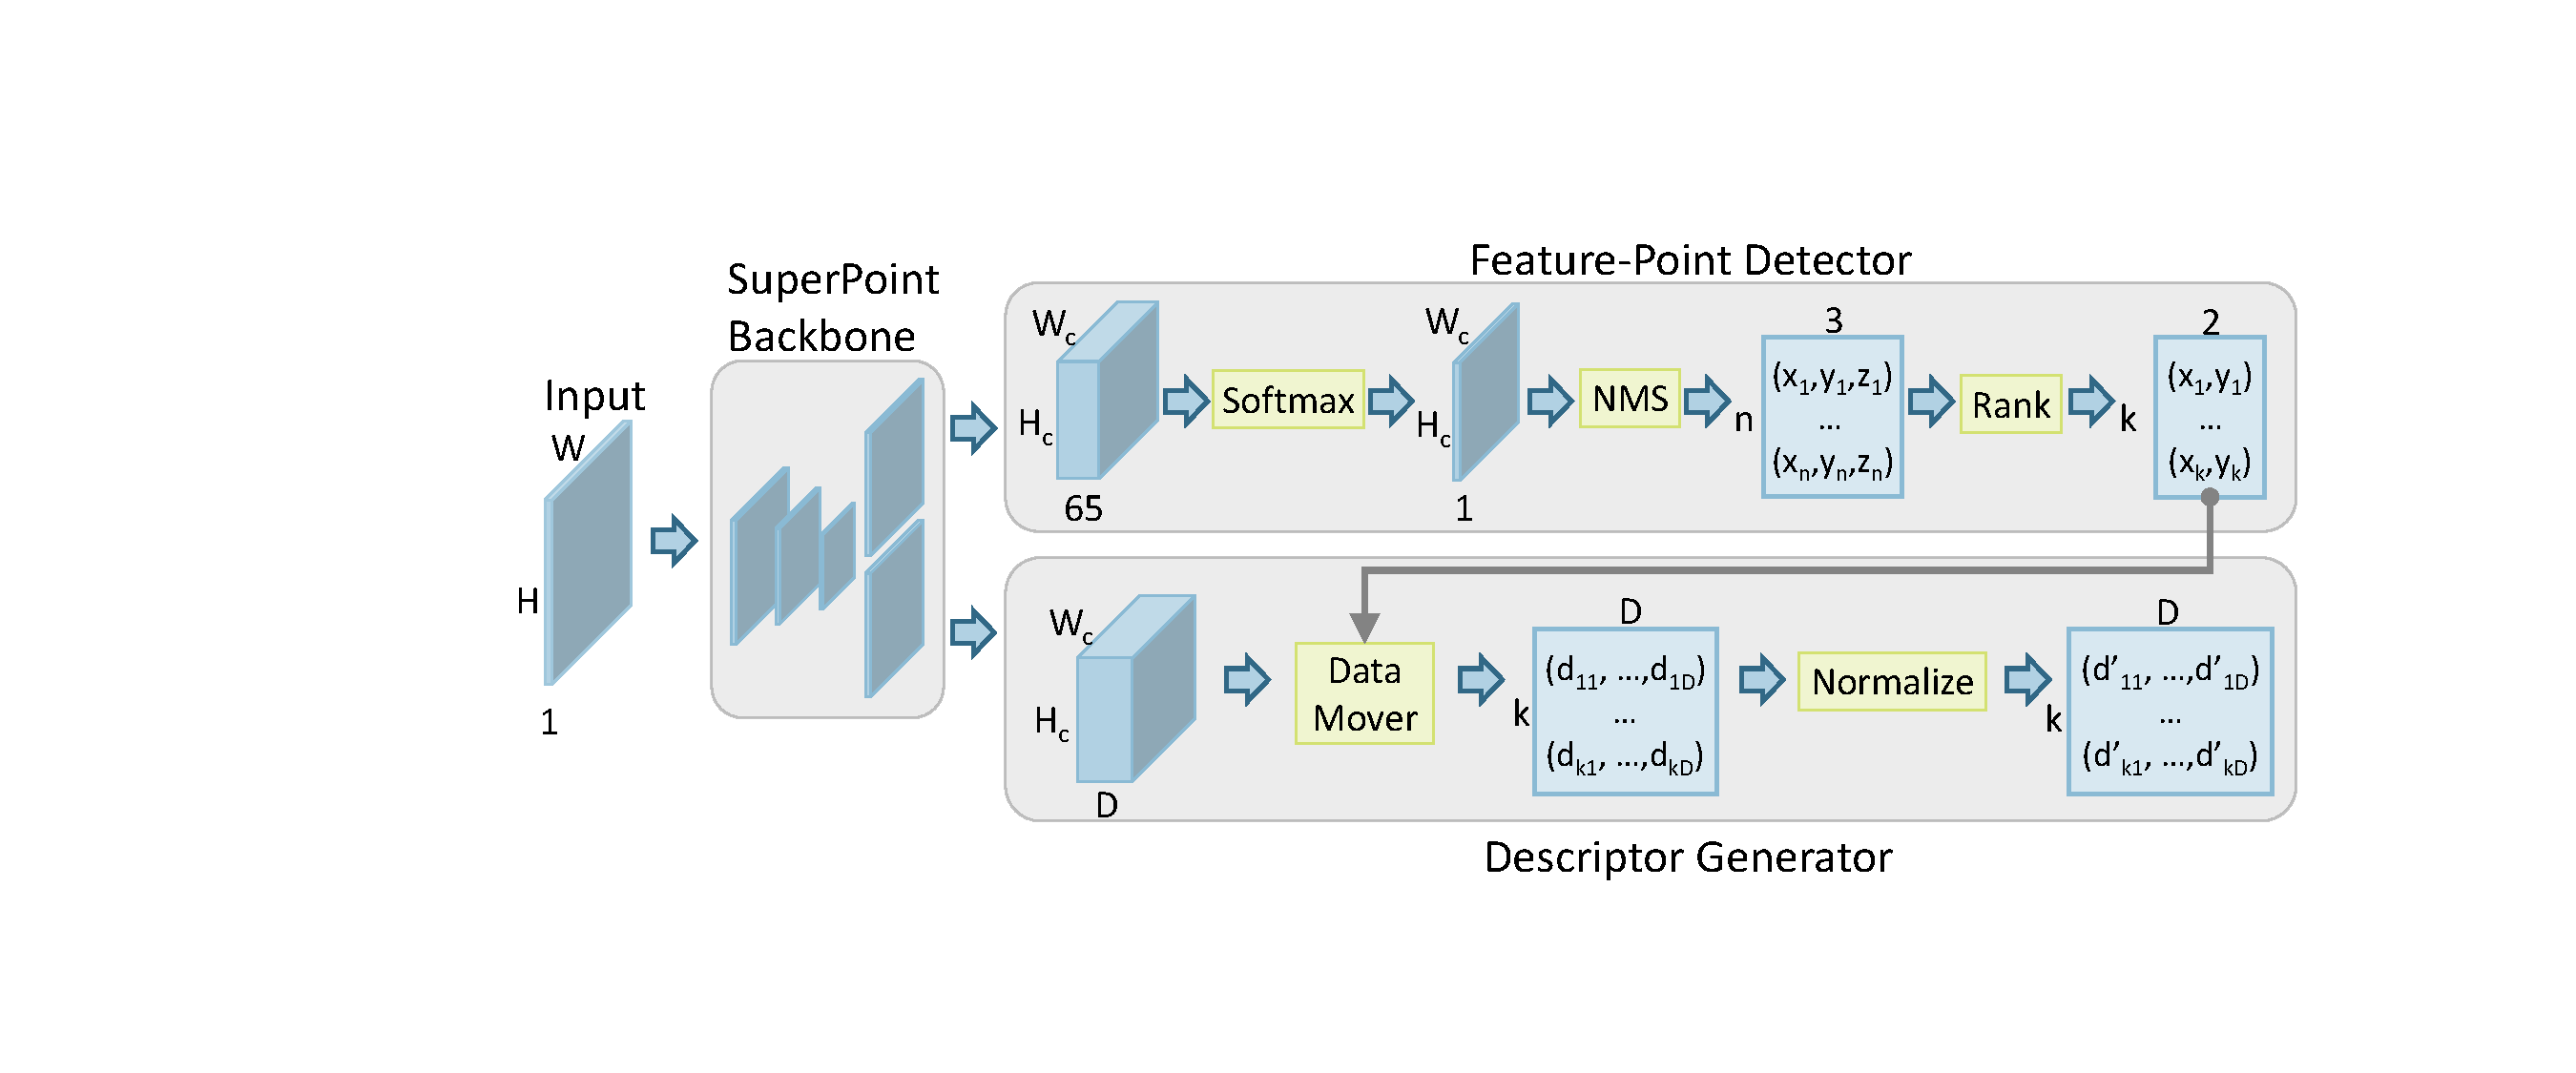
\includegraphics[width=0.99\linewidth]{fig/superpoint.pdf}
    \caption{Optimized feature extraction method based on SuperPoint}
    \label{fig:superpoint}
\end{figure}

As mentioned in \Cref{sec:relate}, there are two steps in the FE method: 1) feature-point detection and 2) feature descriptors generation. 
In SuperPoint \cite{detone2018superpoint}, there are three components in the feature-point detector, 1) Softmax to generate the confidence for each pixel, 2) Non-Maximum Suppression (NMS) to find the pixels with maximum confidence in its neighborhood, 3) Rank component to find out the first $k$ pixels with the highest confidence. 
In the feature descriptors step, the normalization component consumes most of the computation. 

The CNN backbone of SuperPoint maps the input image $I\in \mathbb{R}^{H\times W}$ to a tensor $\mathcal{X}\in \mathbb{R}^{H_c\times W_c\times 65}$ for feature-point detection and to a tensor $\mathcal{D}\in \mathbb{R}^{H_c\times W_c\times D}$ for descriptors generation, where $H_c = H/8$ and $W_c = W/8$.
We optimize the software data flow of the components above, making them less computationally complex and friendly to hardware. 
The flow path of our SuperPoint-based feature extraction method is shown \Cref{fig:superpoint}. 
Then we design FPGA accelerators specifically for calculating softmax and normalization.

\subsection{Softmax Optimization}
\label{sec:softmaxopt}

\begin{figure}[t]
    \centering  
    \vspace{-0.1cm} 
    \setlength{\abovecaptionskip}{0cm} 
    \setlength{\belowcaptionskip}{-0.05cm} 
    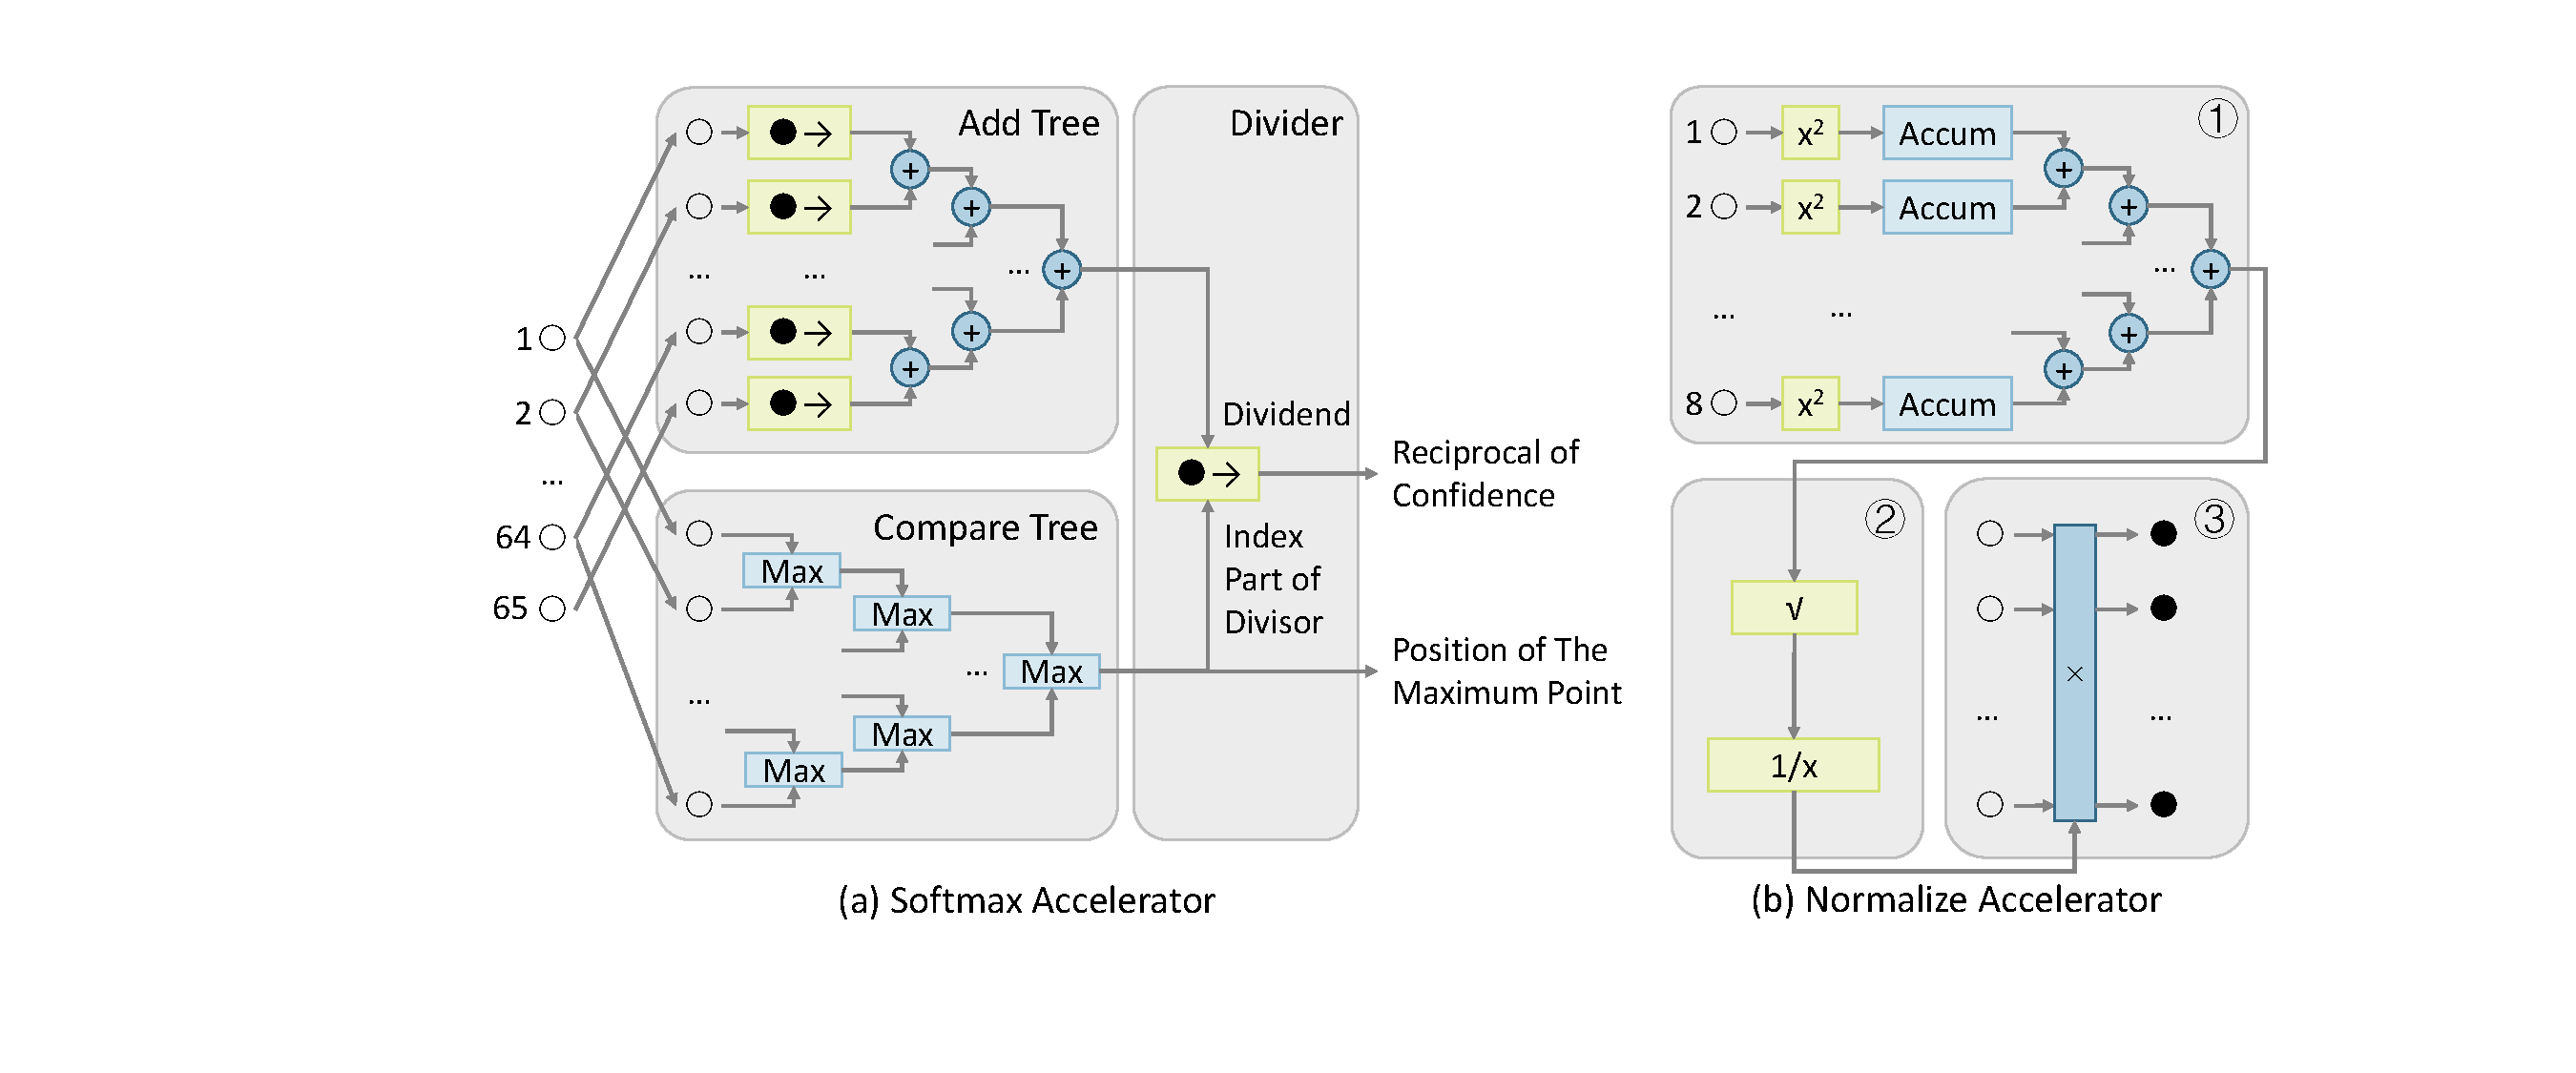
\includegraphics[width=0.99\linewidth]{fig/FEaccelerator.pdf}
    \caption{Hardware Architecture of FE Accelerators}
    \label{fig:FEaccelerator}
\end{figure}

For feature-point detection, the 65 channels correspond to local, non-overlapping $8 \times 8$ pixel grid areas plus a background channel. 
After a channel-wise softmax, the background channel is removed, and a $\mathbb{R}^{H_c\times W_c\times64}\Rightarrow \mathbb{R}^{H\times W}$ reshaping is performed. 
The channel-wise softmax makes the points in different grid areas have equal confidences.
The tensor of size $\mathbb{R}^{H\times W}$ corresponds to the confidences of the feature points in the input image.

The standard softmax function is defined as $\sigma (\mathbf {z} )_{i}$ in \Cref{equ:softmax_hard}.
We optimize the process of softmax that we only take the maximum value of each grid area for subsequent computations, which not only reduces the division operations of softmax but also simplifies the calculation of NMS and Rank.
We reduce the division operations and output size of softmax from $H \times W$ to $H_c \times W_c$.
The division operation is resource consuming on FPGA platforms. 
Our method can greatly reduce the number of divisions by $64 \times$, making it easy to accelerate softmax operation on FPGA.

\begin{equation}
    \sigma (\mathbf {z} )_{i}={\frac {e^{z_{i}}}{\sum _{j=1}^{K}e^{z_{j}}}}
    \Rightarrow
    \frac{1}{\sigma (\mathbf {z} )_{i}}={\frac {\sum _{j=1}^{K}2^{z_{j}}}{2^{z_{i}}}}{\text{ for }}i=1,\dotsc ,64;
    \label{equ:softmax_hard}
\end{equation}

Since the results of the softmax function are all positive, we can calculate the reciprocal of the softmax function ($\frac{1}{\sigma (\mathbf {z} )_{i}}$) in \Cref{equ:softmax_hard} as the normalized confidence, without affecting the results of the NMS and ranking process. We quantize the output feature map of CNN to 8-bit fixed-point integer, i.e each $z_i$ in \Cref{equ:softmax_hard} is a 8-bit fixed-point integer. We change the base of the power from $e$ to $2$ to make it hardware friendly. Since the divisor is a power of $2$, we can also implement division by shift operation.

\Cref{fig:FEaccelerator}(a) shows an overview of the softmax module. It consists of three parts, add tree, compare tree and divider. Softmax reads 65 numbers from a grid region at once. Add tree computes input to the power of $2$ using shift operation and calculates their sum. Compare tree reads the values of the first 64 channels and returns the maximum value and its channel number which contains position information. The divider uses the shift operation to calculate the reciprocal of confidence.

\subsection{NMS Optimization}

Non-maximum suppression(NMS) is applied to the detection to help ensure that the feature-points are evenly distributed throughout the image. 
For each pixel in the original input image, NMS compares the confidence of this pixel with that of the pixels in a square neighborhood whose edge including $\epsilon _{ori}$ pixels. 
If the confidence of the target central pixel is not the maximum in its neighbors, this point will be eliminated from the valid feature-points. 
The output of the NMS is a list of coordinates and confidences for each feature-point. 
There are totally $H \times W$ points and the NMS does $\epsilon _{ori} ^ 2 - 1$ comparison operations for each points. 
Thus, in the original NMS method, there are totally $H \times W \times (\epsilon _{ori} ^ 2 - 1)$ comparison operations.

The softmax optimization introduced in \Cref{sec:softmaxopt} already gives the pixel with maximum confidence of each $8 \times 8$ block. Thus, we only need to compare each output pixel of softmax to the its adjacent blocks. The comparison area is a square box with an edge of $\epsilon _{opt}$ pixels. and $\epsilon _{opt} = 2\times \left \lceil (\epsilon _{ori}-1)/16 \right \rceil +1$. There are only $H_c \times W_c$ points. Thus, after NMS optimization, there are totally $H_c \times W_c \times (\epsilon _{opt} ^ 2 - 1)$ comparison operations.

The $\epsilon _{ori}$ is set to 9 in the original implements SuperPoint, so $\epsilon _{opt} = 2\times \left \lceil (\epsilon _{ori}-1)/16 \right \rceil +1 = 3$. So that $H \times W \times 80 $ comparisons are done in the original NMS and we can do only $H_c \times W_c \times 8$ comparisons after optimization. The total number of comparisons is reduced by $640\times$.

\subsection{Ranking Optimization}

The ranking operation is to find out the top $k$ feature-points with maximum confidence. 
The output is a list of coordinates for the $k$ feature-points. 
In the original implementation, the confidence of all valid feature-points after NMS is sorted, and only the first $k$ feature points are used in the applications like SLAM and image matching. 
There are $N_{nms}$ valid points after NMS. To sort all these $N_{nms}$ points, the time complexity is defined as:

\begin{equation}
    C_{sort} = O(N_{nms} \cdot log(N_{nms}))
    \label{equ:csort}
\end{equation}

We create a heap of size $k$ and then look for the $k$ feature-points with the highest confidence. We do not compute the order of these $k$ points. The time complexity of the optimized ranking method is:

\begin{equation}
    C_{heap} = O(N_{nms} \cdot log(k))
    \label{equ:optsort}
\end{equation}

In our expetiments, $N_{nms} \approx 2000$ and $k = 200$. The number of comparisons is reduced by $1.4\times$.

\subsection{Normalization Optimization}

The input of the descriptor head sized $\mathbb{R}^{H_c\times W_c\times D}$ is semi-dense descriptor that each $8\times8$ pixel cell has a descriptor. In the original implementation, a bicubic interpolation and normalization yields fine descriptors of size $\mathbb{R}^{H\times W\times D}$. Then, according to the result of the rank, the descriptors corresponding to the k feature points are combined into a list and output. When using maximum point softmax, each $8\times8$ pixel cell only has a potential feature-point. So we can use semi-dense descriptor as the dense descriptor of the potential feature-point and do not need bi-cubic interpolation.

The number of descriptors that need to be normalized has been reduced from $H\times W$ to $H_c\times W_c$. In addition, we normalize the descriptors after sorting the feature-points, which means we only need to normalize $k$ descriptors. If we set $H=480$, $W=640$ and $k=200$, then the computational complexity of the normalization process will be reduced by $1500\times$. However, $k$ descriptors are not stored in contiguous memory space. We use a datamover to move data from discrete address spaces.

The architecture of normalization accelerator is illustrated in \Cref{fig:FEaccelerator}(b). The normalization module can read 8 numbers per clock cycle. The normalization process is divided into three stages and requires each descriptor to be read twice. In the first stage, we compute the sum of the squares of the descriptors, which takes 32 clock cycles when $D=256$. Then the reciprocal of square root of sum is computed as the normalization coefficient. In the final stage, the descriptor is read a second time and multiplied by the normalization coefficient.

% \subsection{Optimization for PR Post-Processing}

% \begin{figure}[t]
%     \centering
%     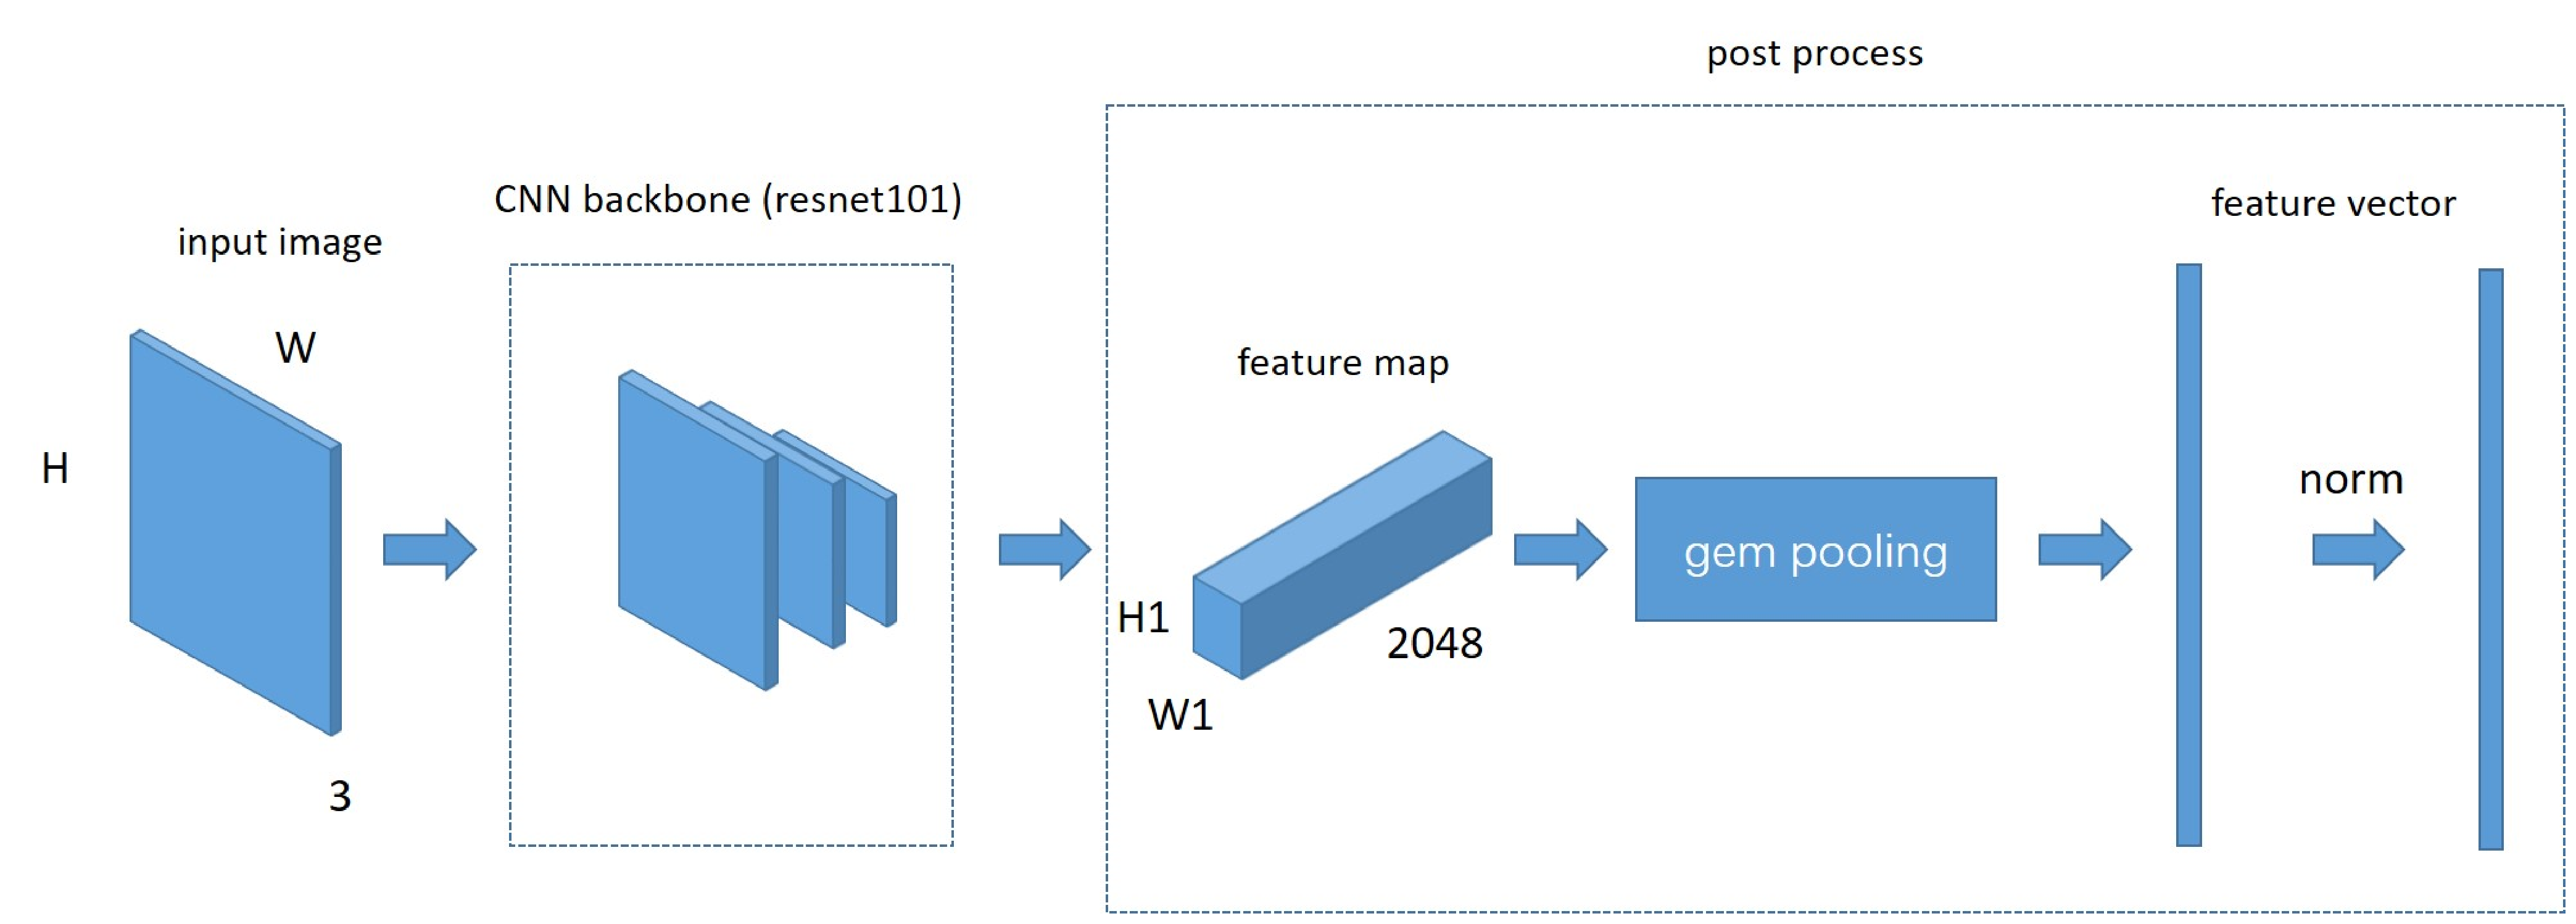
\includegraphics[width=1\linewidth]{fig/pr.eps}
%     \caption{The architecture of GeM network}
%     \label{fig:gem}
% \end{figure}

% Figure \ref{fig:gem} shows the data flow of GeM network \cite{gem} for PR. The CNN backbone of GeM is a resnet101 network without the last two layers(pooling and FC). The CNN maps the input image $ I \in \mathbb{R}^{3 \times H \times W}$ to a tensor $\mathcal{X} \in \mathbb{R}^{C \times H_1 \times W_1}$. Here, the channel number $C = 2048$. Then the gem pooling layer pool the tensor into a vector $\mathcal{V} \in \mathbb{R}^{C}$. (To avoid ambiguity, we use "GeM" to represent the whole network and "gem" to represent the pooling layer only.) Finally, the vector is normalized. After that, we use dot product or L2 distance of the vectors to calculate similarity of places. Because feature extraction needs to be real-time and is time consuming, we modify its software utilization and design FPGA accelertor for this process.

% Experiments show that the post processing (gem pooling and normalization) consume nearly twice the time as CNN network does. After optimization, we can reduce time to 1/? of that of origin.

% \subsubsection{GeM Pooling Optimization}

% The element of the vector $\mathcal{V}$ is calculated by

% \begin{equation}
%     \mathcal{V}_i = (\sum_{x \in \mathcal{C}_i} x^p)^{1/p}, i=1, 2, ..., 2048.
% \end{equation}

% Here, the parameter $p$ is learned by back propagation and is set to 2.9? in original paper. To make it friendly for hardware computation, we change it to $p=3$. In this way, the power computation can be converted to multiplication computation. This will save a lot of time and calculation resources on FPGA without loss of accuracy. We notice that the channels are independent with each other, so it's convenient to do parallel computation on FPGA. With Vivado HLS tool, we design an IP core for gem pooling and efficiently reduce time.

% \subsubsection{Normalization Optimization}